% Appendix A

\chapter{Model Summaries} % Main appendix title

\label{AppendixA} % For referencing this appendix elsewhere, use \ref{AppendixA}

\section{Summary of Models of Experiment 1}

Below summaries of models used in Experiment 1 are shown.

\subsection{Supervised Learning}

Figure \ref{fig:summary_CNN_class_syn} shows the summary of the CNN classification model of Experiment 1. The models consists of two convolutional layers with 32 neurons, two max pooling layers, a flatten layer, a dense layer with 16 neurons and the output layer with 1 neuron. 
\begin{figure}[h]
	\centering
	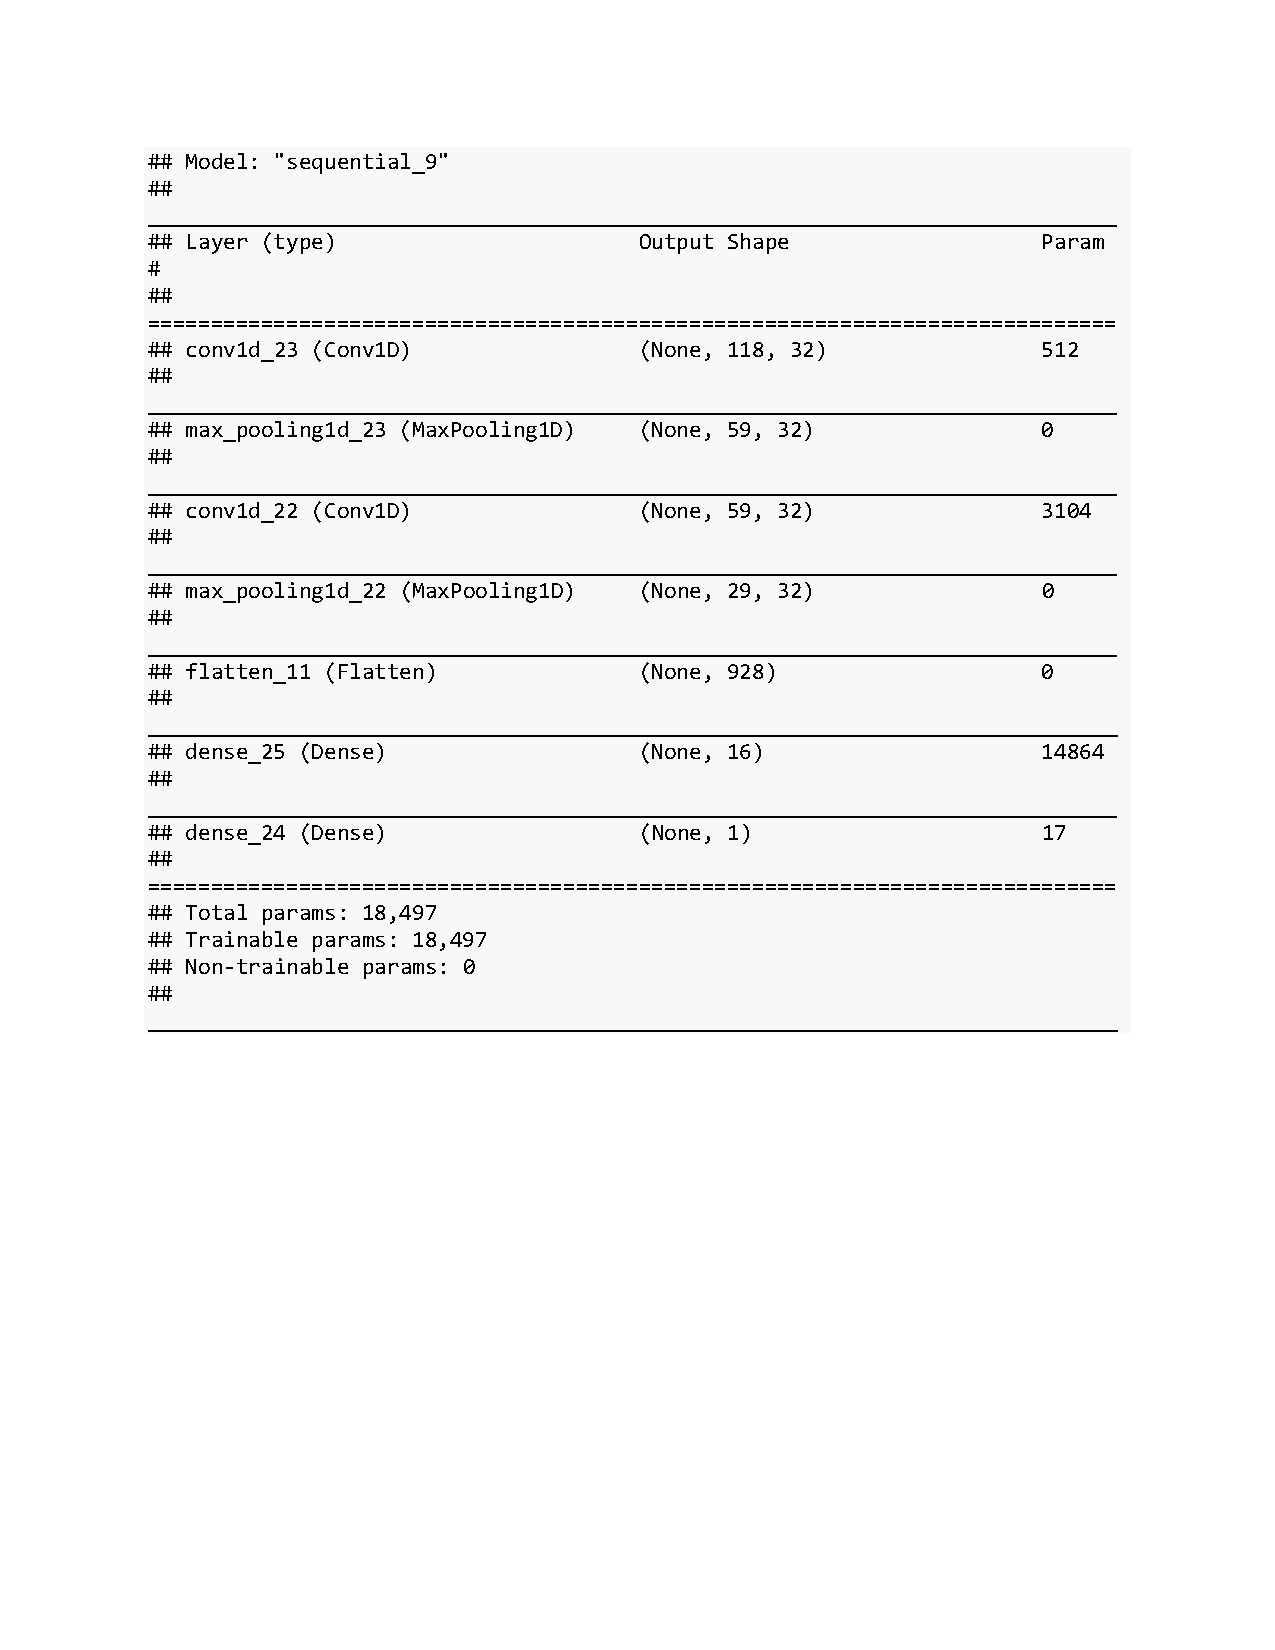
\includegraphics[scale=0.45]{Figures/summary_CNN_class_syn}
	\decoRule
	\caption[Experiment 1: Summary of CNNs for supervised learning]{Summary of CNN \parencite{own}}
	\label{fig:summary_CNN_class_syn}
\end{figure}

Figure \ref{fig:summary_GRU_class_syn} shows the summary of the RNN classification model used in Experiment 1. The model consists of two GRU layers with 32 neurons, a dense layer with 16 neurons and the output layer with 1 neuron. 

\begin{figure}[h]
	\centering
	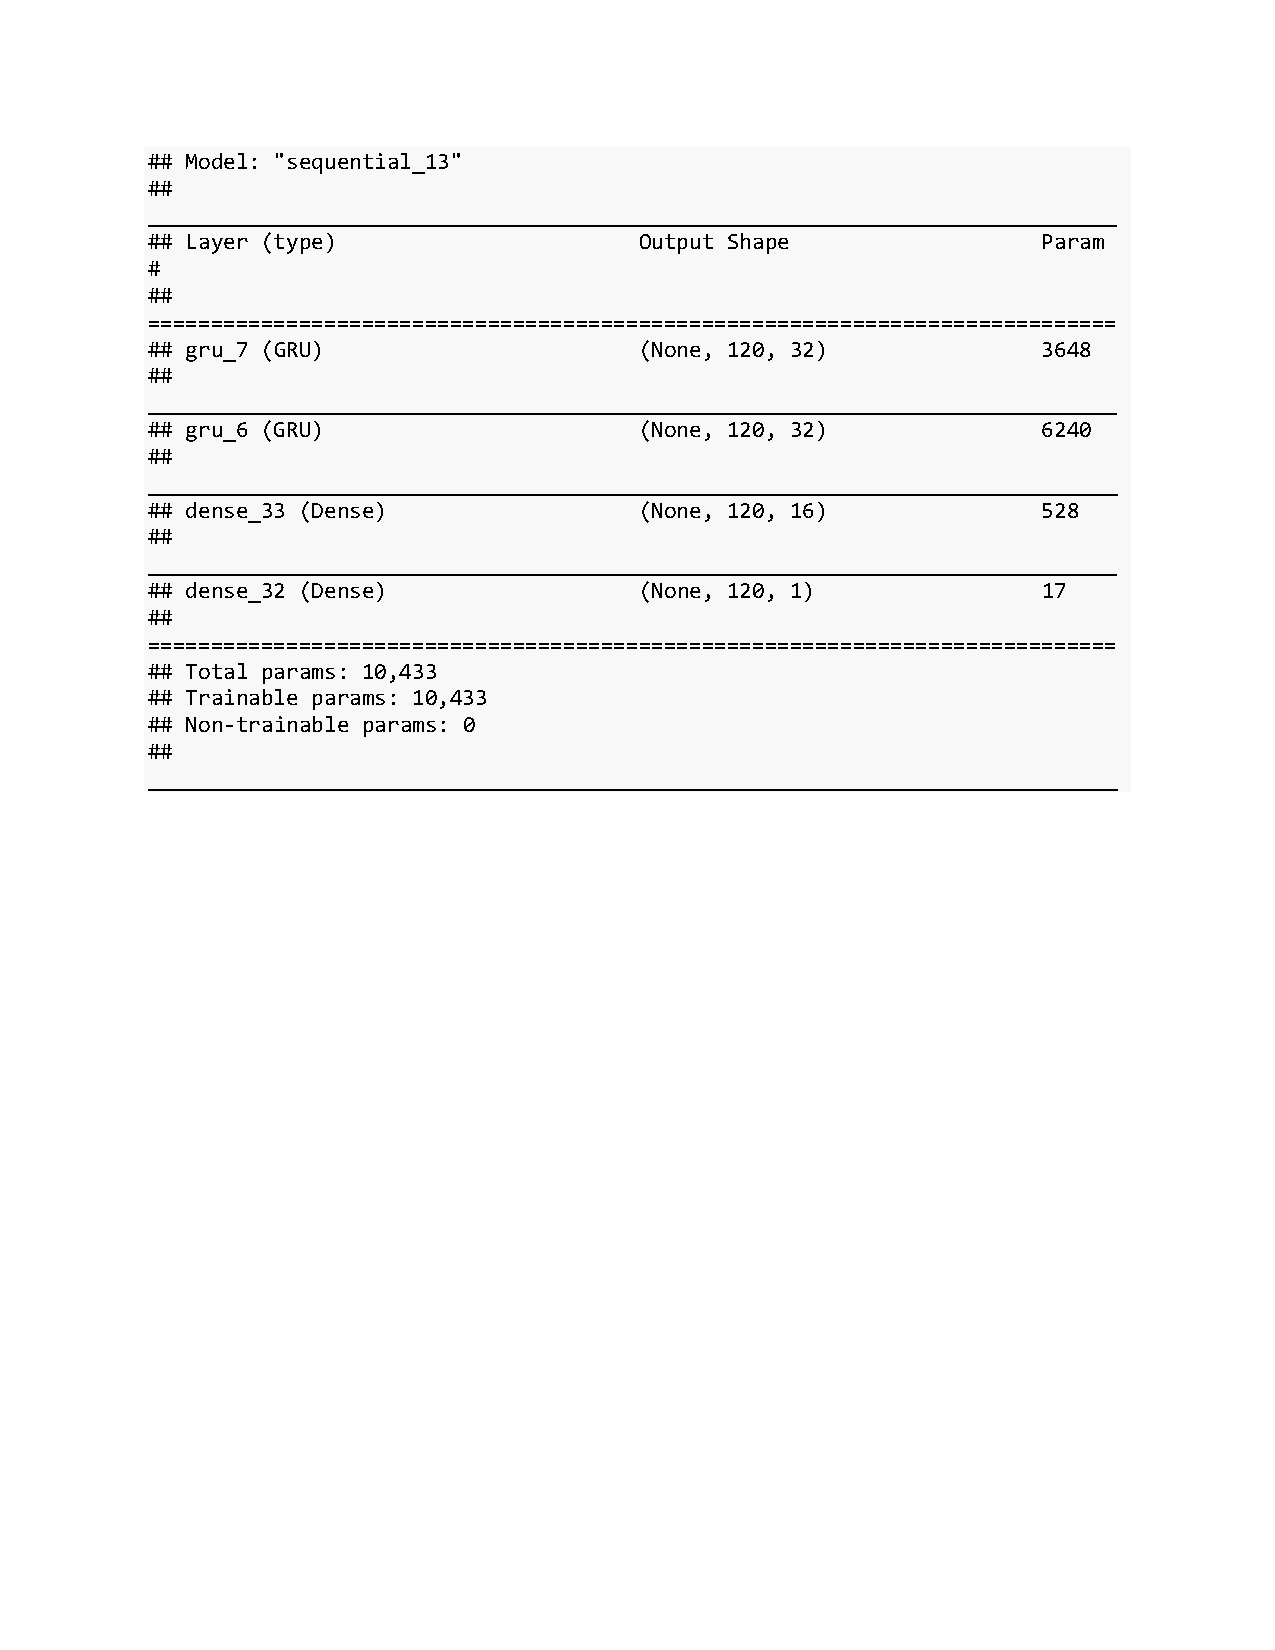
\includegraphics[scale=0.5]{Figures/summary_GRU_class_syn}
	\decoRule
	\caption[Experiment 1: Summary of GRU for supervised learning]{Summary of GRU \parencite{own}}
	\label{fig:summary_GRU_class_syn}
\end{figure}

\clearpage
\subsection{Unsupervised Learning}

Figure \ref{fig:summary_CNN_pred_syn} shows the summary of the CNN predictive model used in Experiment 1. The model consists of two convolutional layers with 32 neurons, two max pooling layers, a flatten layer, and five output layer with 1 neuron each. 
\begin{figure}[h]
	\centering
	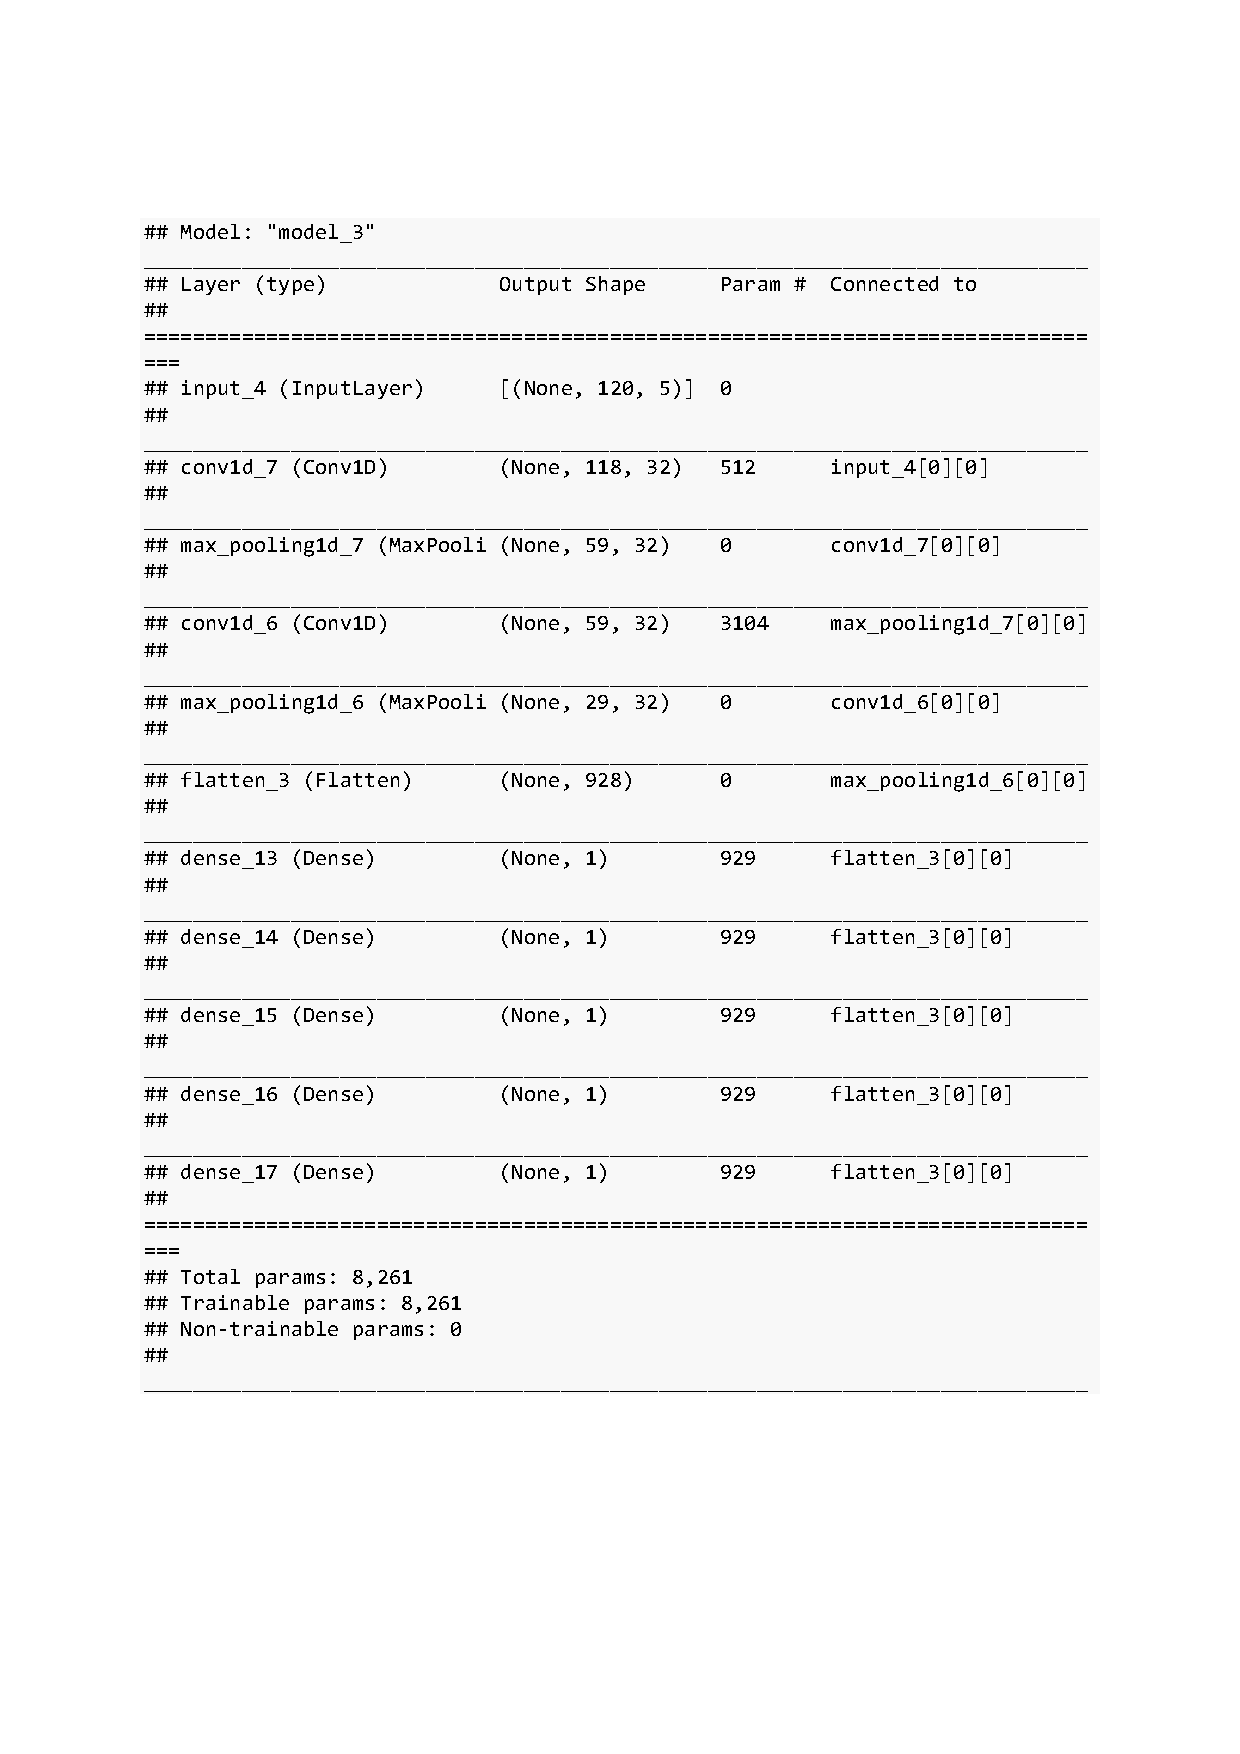
\includegraphics[scale=0.5]{Figures/summary_CNN_pred_syn}
	\decoRule
	\caption[Experiment 1: Summary of CNN for unsupervised learning]{Summary of CNN \parencite{own}}
	\label{fig:summary_CNN_pred_syn}
\end{figure}
\clearpage
Figure \ref{fig:summary_GRU_pred_syn} shows the summary of the RNN predictive model used in Experiment 1. The model consists of two GRU layers with 32 neurons and the output layers with 5 neurons.  
\begin{figure}[h]
	\centering
	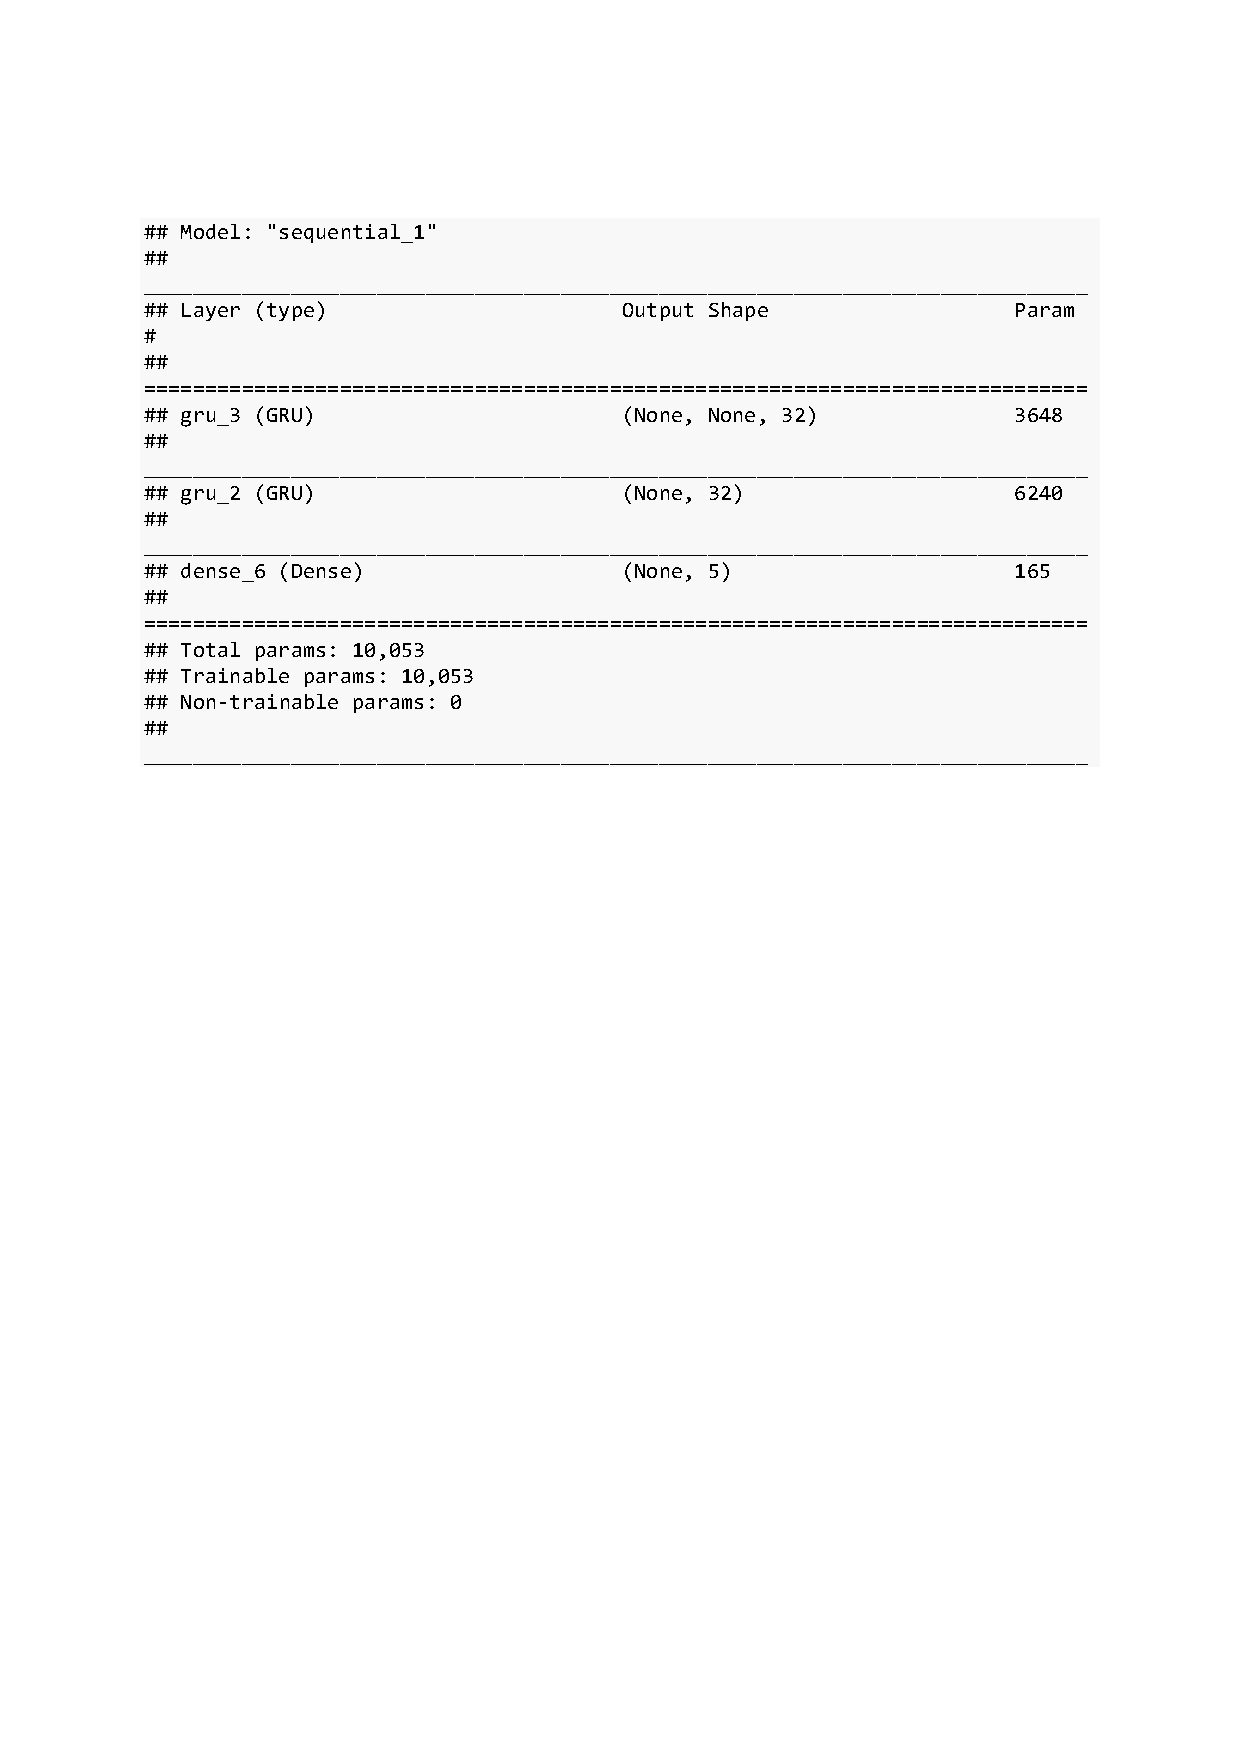
\includegraphics[scale=0.5]{Figures/summary_GRU_pred_syn}
	\decoRule
	\caption[Experiment 1: Summary of GRU for unsupervised learning]{Summary of GRU \parencite{own}}
	\label{fig:summary_GRU_pred_syn}
\end{figure}

\clearpage

\section{Summary of Models of Experiment 2} \label{exp2_summary}

Below summaries of models used in Experiment 2 are shown.

\subsection{Supervised Learning}
Figure \ref{fig:CNN_classifier_house_temp} shows the summary of the CNN classification model of Experiment 2. The models consists of two convolutional layers with 32 neurons, two max pooling layers, a flatten layer, a dense layer with 16 neurons and the output layer with 1 neuron.
\begin{figure}[h]
	\centering
	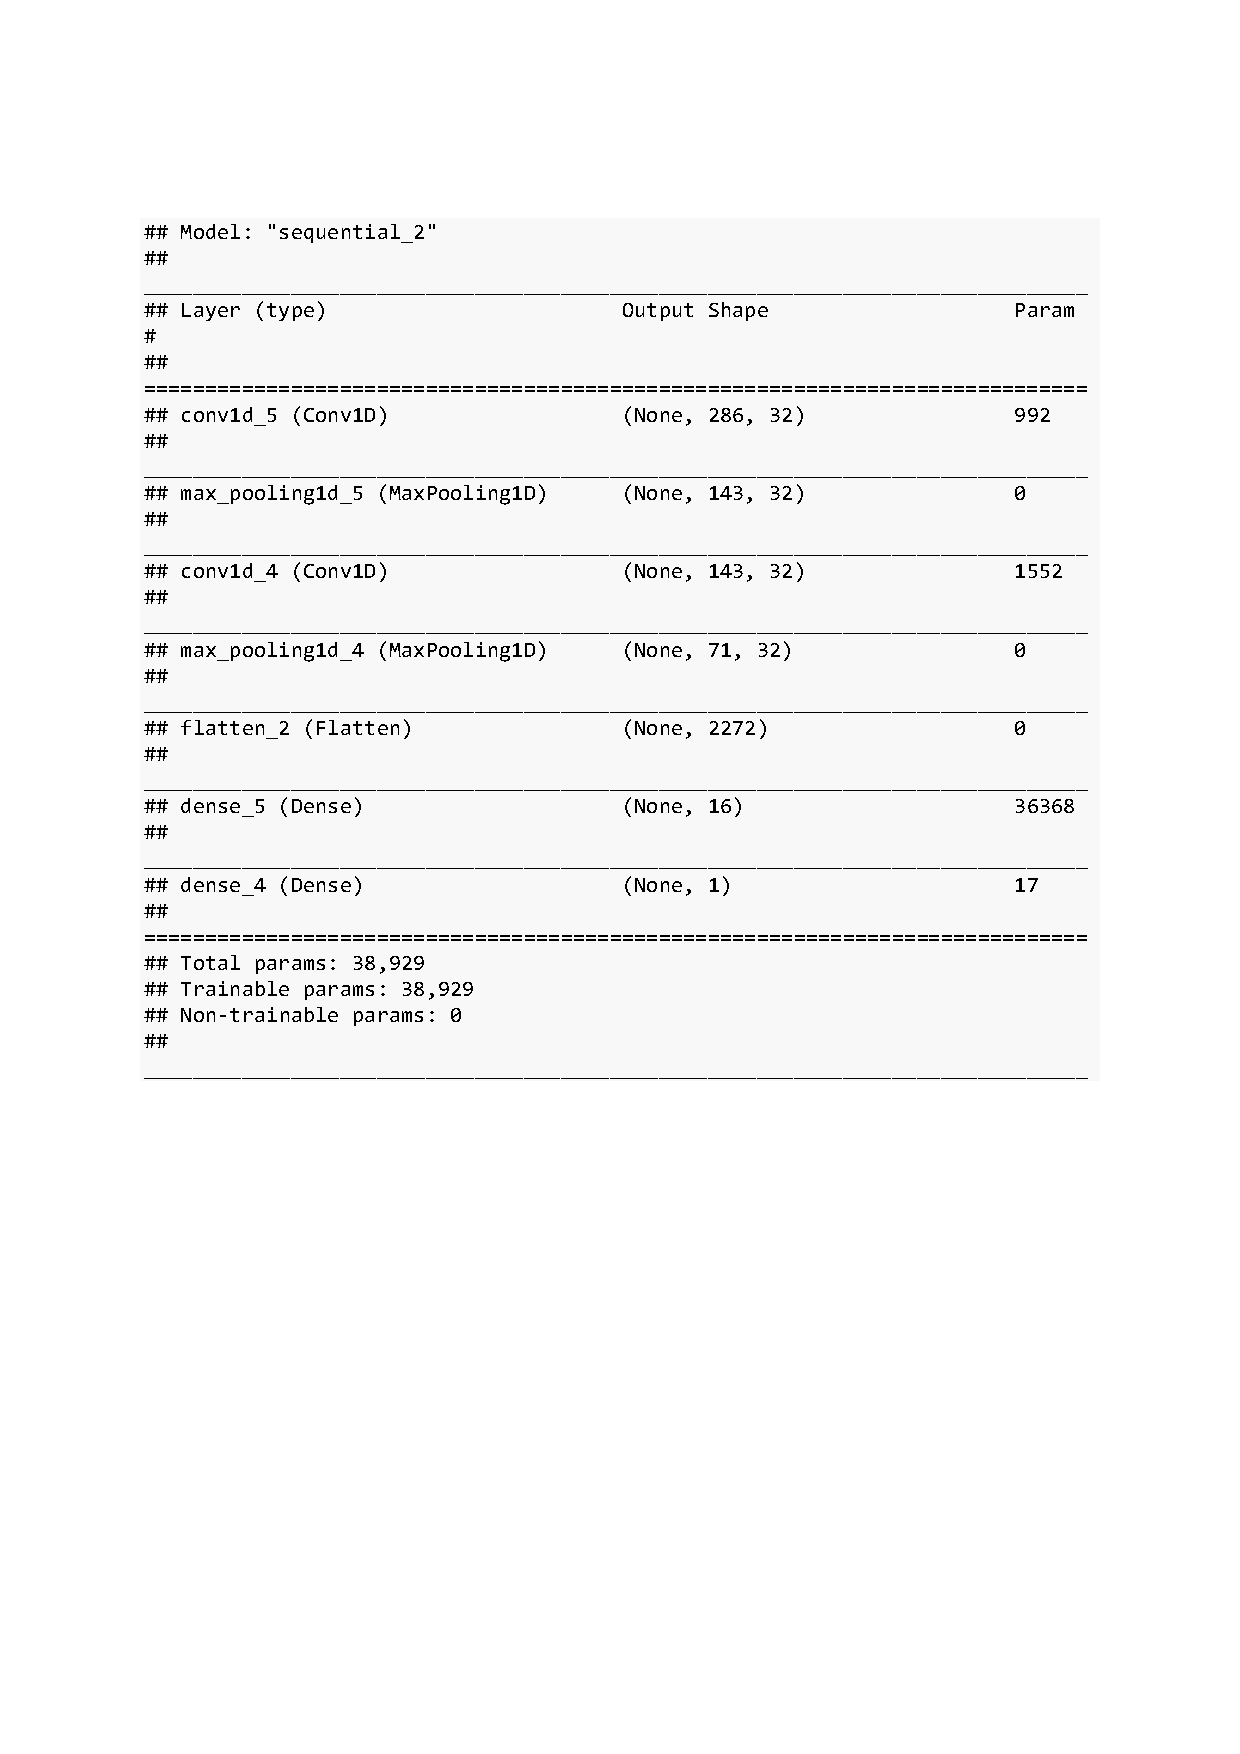
\includegraphics[scale=0.5]{Figures/summary_CNN_class_house_temp}
	\decoRule
	\caption[Experiment 2: Summary of CNN for supervised learning]{Summary of CNN \parencite{own}}
	\label{fig:CNN_classifier_house_temp}
\end{figure}
\clearpage
\subsection{Unsupervised Learning}

Figure \ref{fig:summary_CNN_pred_house_temp} shows the summary of the CNN predictive model used in Experiment 2. The model consists of three convolutional layers, one max-pooling layer, a flatten layer and four output layers with 1 neuron.
\begin{figure}[h]
	\centering
	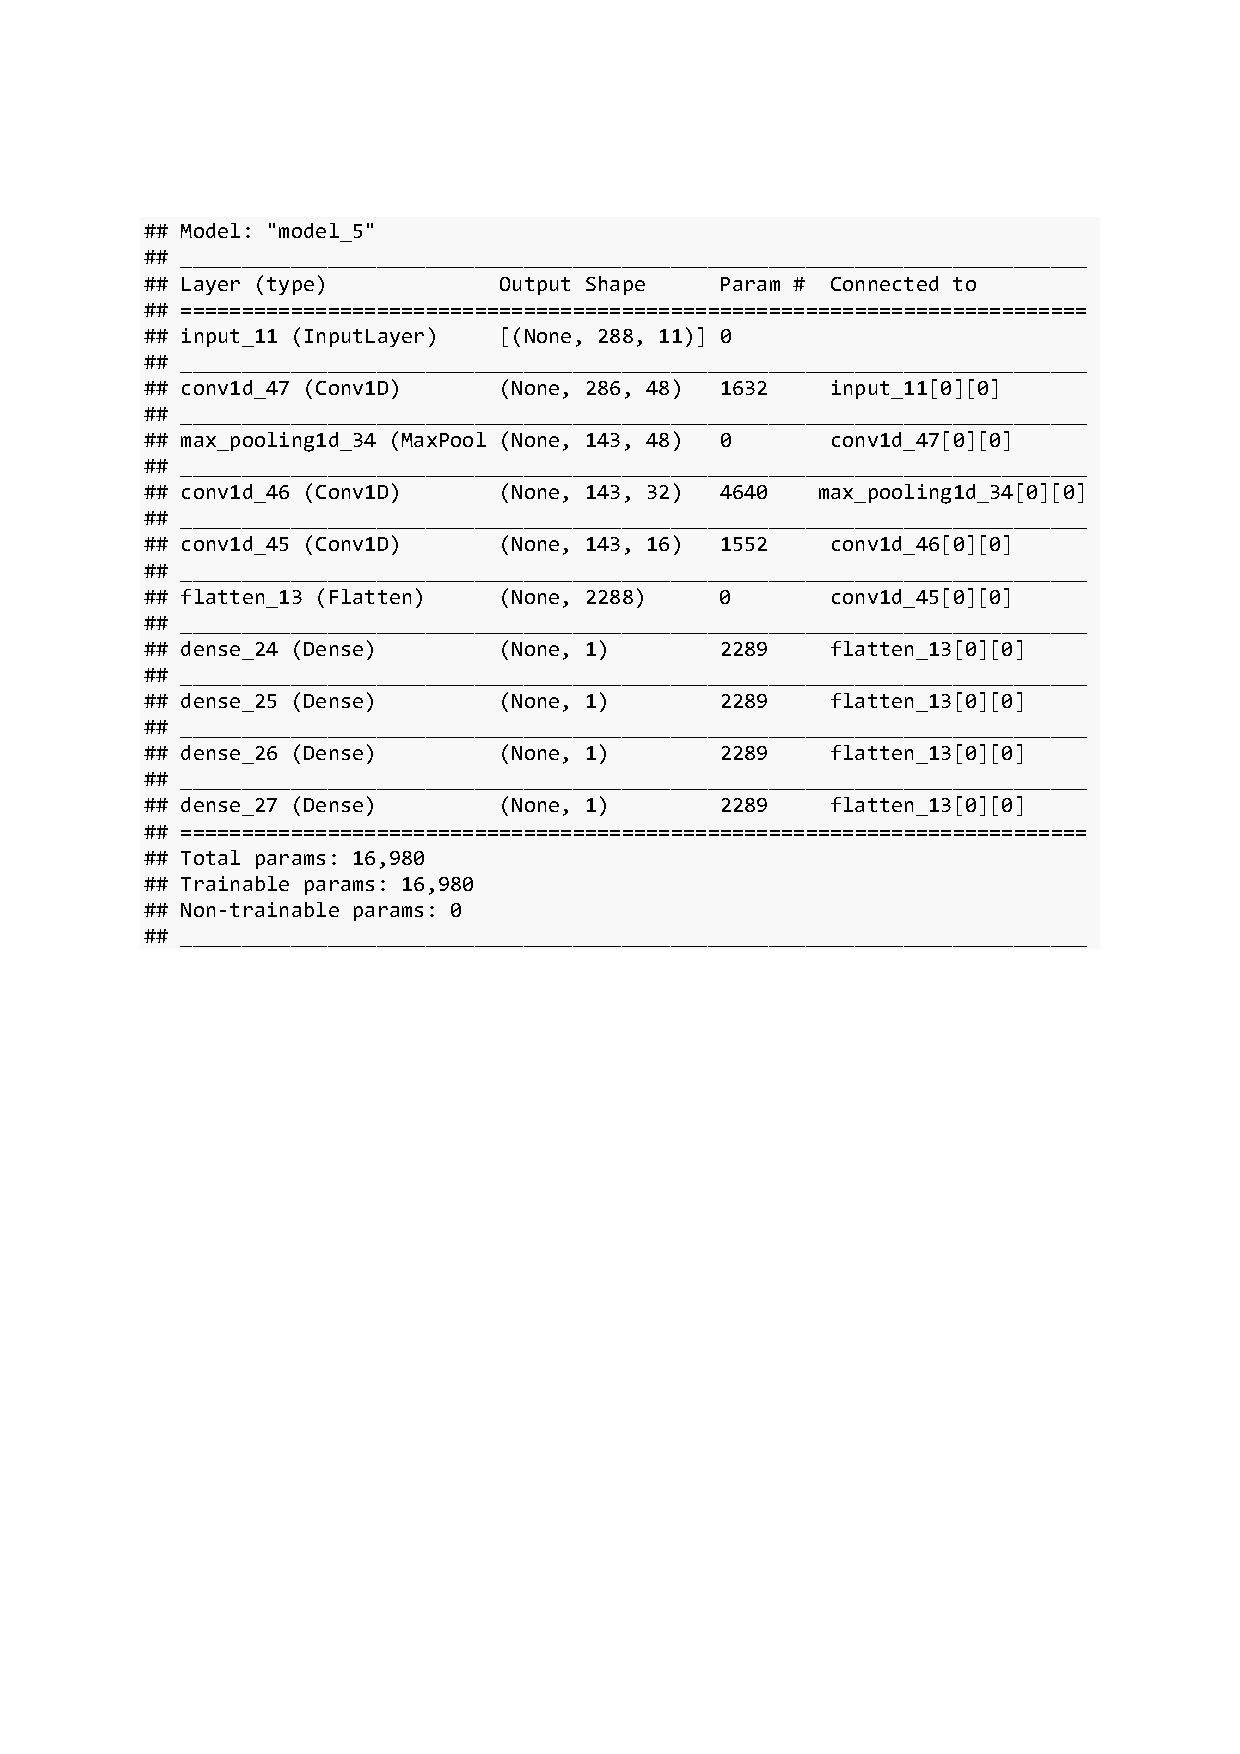
\includegraphics[scale=0.5]{Figures/summary_CNN_pred_house_temp}
	\decoRule
	\caption[Experiment 2: Summary of CNN for unsupervised learning]{Summary of CNN \parencite{own}}
	\label{fig:summary_CNN_pred_house_temp}
\end{figure}
\clearpage
Figure \ref{fig:summary_LSTM_pred_house_temp} shows the summary of the RNN predictive model used in Experiment 2. The model consists of three LSTM layers and the output layer with 4 neurons.
\begin{figure}[h]
	\centering
	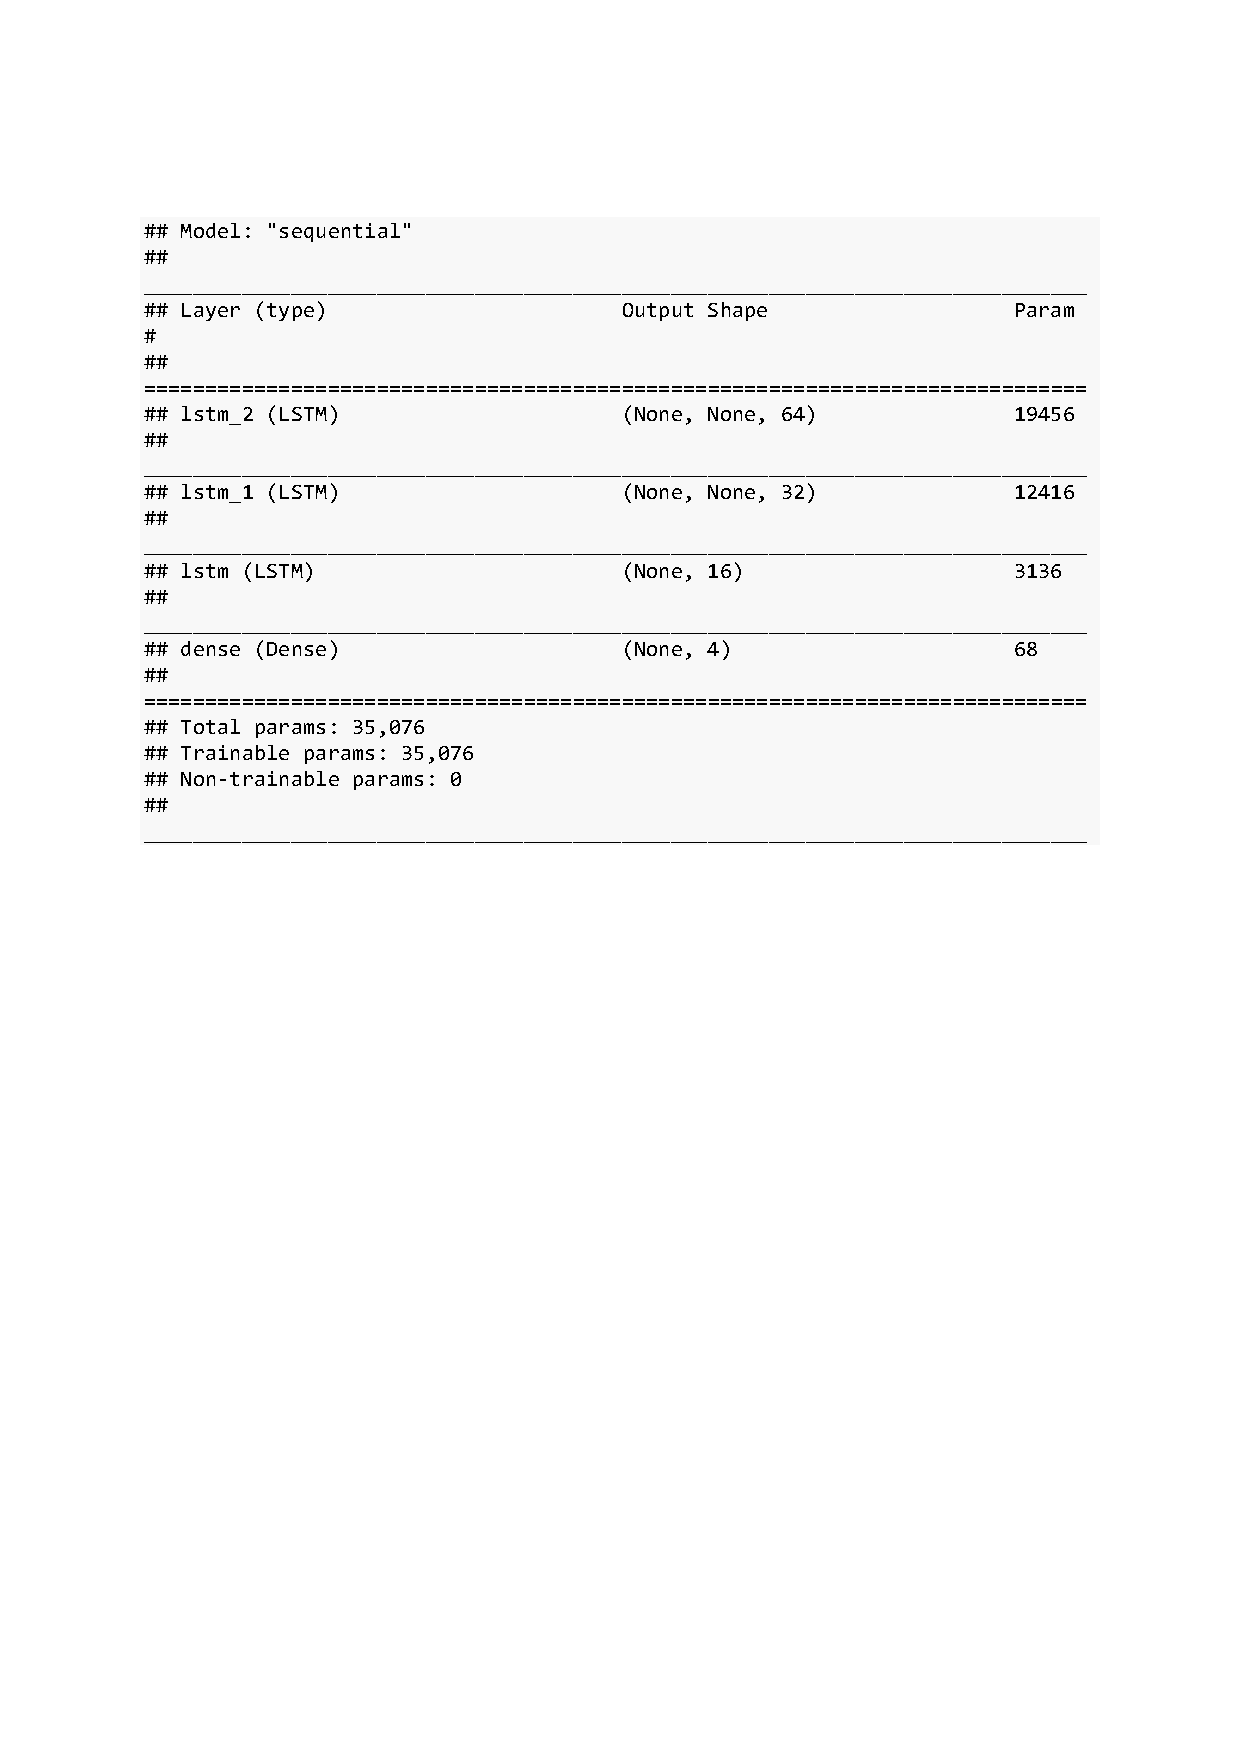
\includegraphics[scale=0.5]{Figures/summary_LSTM_pred_house_temp}
	\decoRule
	\caption[Experiment 2: Summary of LSTM for unsupervised learning]{Summary of LSTM \parencite{own}}
	\label{fig:summary_LSTM_pred_house_temp}
\end{figure}

\clearpage
\section{Summary of Models of Experiment 3}


Below summaries of models used in Experiment 3 are shown.


\subsection{Unsupervised Learning}
Figure \ref{fig:summary_CNN_GHL} shows the summary of the CNN predictive model used in Experiment 3. The model consists of three convolutional layers, two dropout layers, a flatten layer and two output layers with 1 neuron.
\begin{figure}[h]
	\centering
	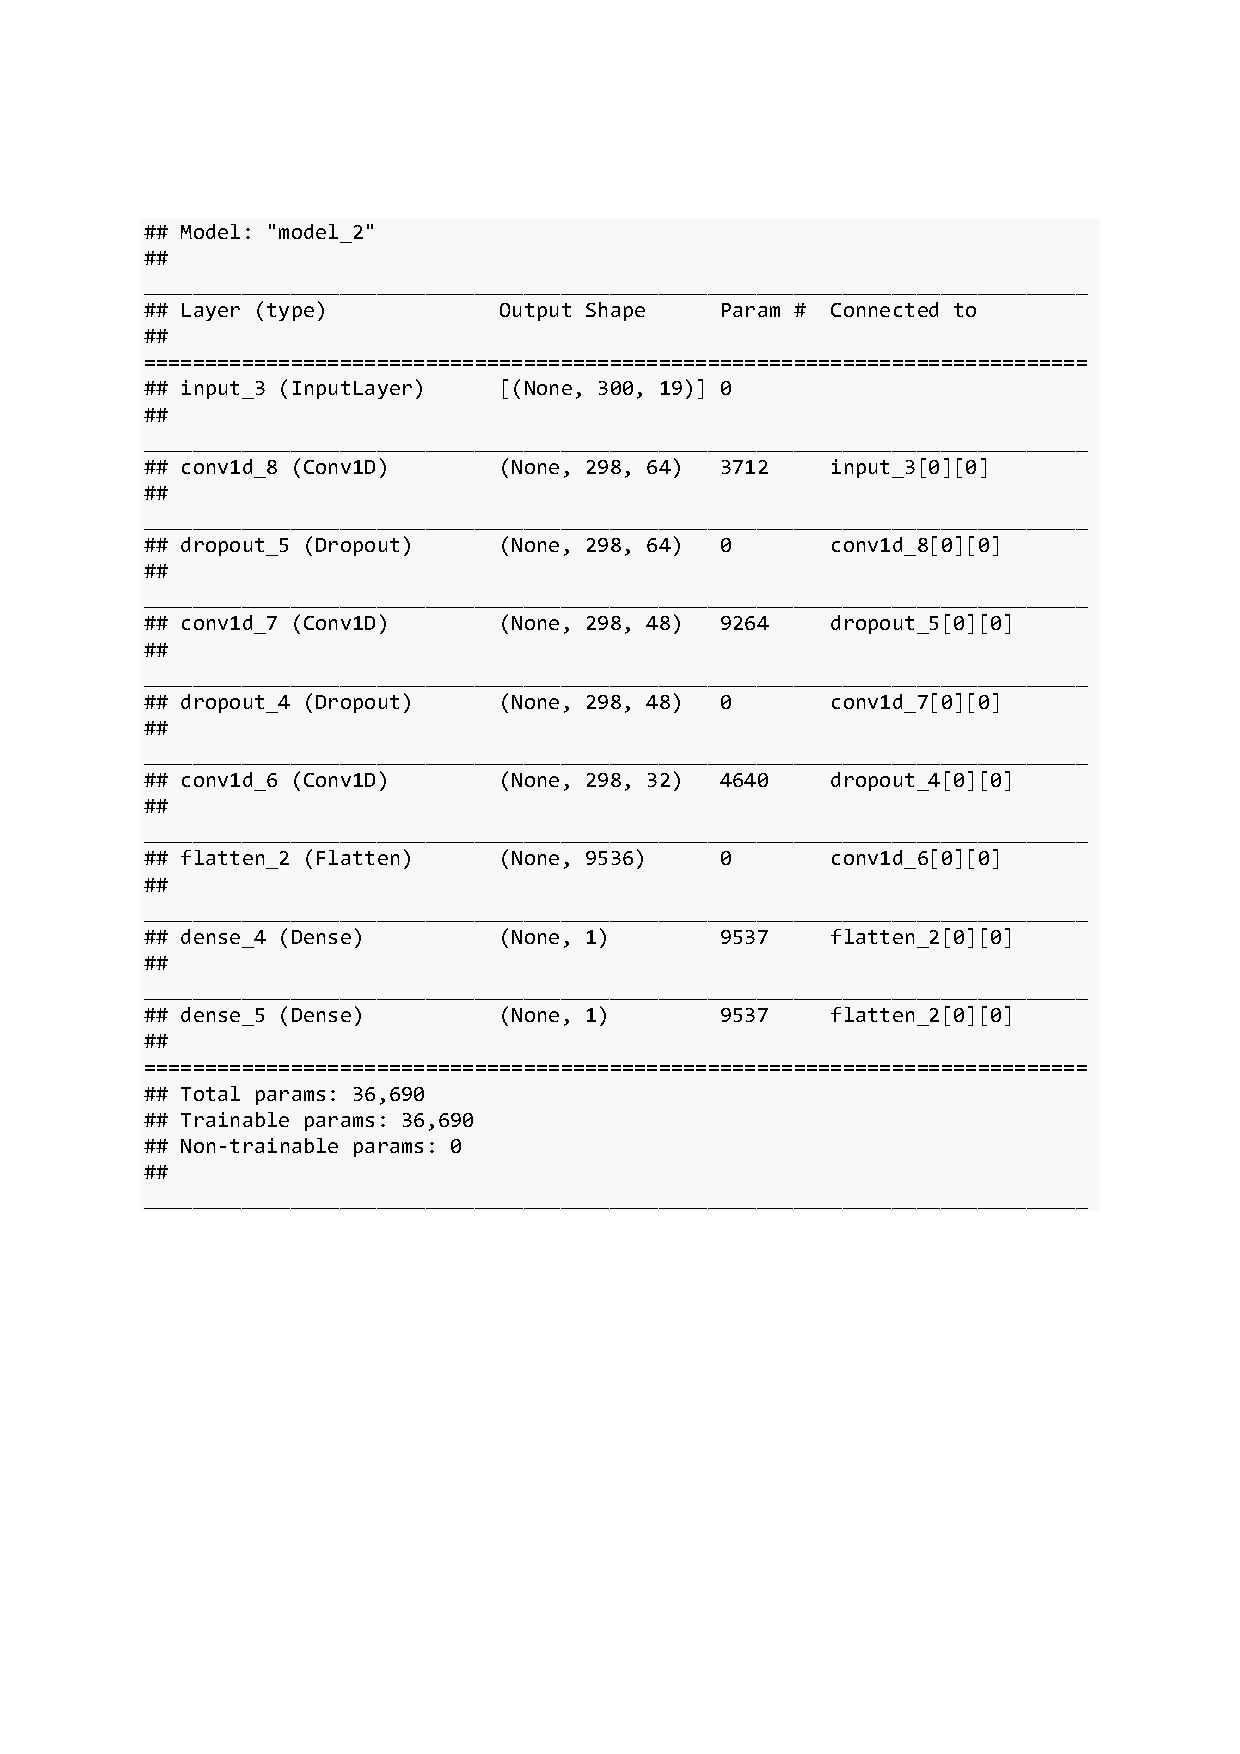
\includegraphics[scale=0.5]{Figures/summary_CNN_GHL}
	\decoRule
	\caption[Experiment 3: Summary of CNN for unsupervised learning]{Summary of CNN \parencite{own}}
	\label{fig:summary_CNN_GHL}
\end{figure}
\clearpage
Figure \ref{fig:summary_LSTM_GHL} shows the summary of the RNN predictive model used in Experiment 3. The model consists of two LSTM layers, a dropout layer and the output layer with 2 neurons.
\begin{figure}[h]
	\centering
	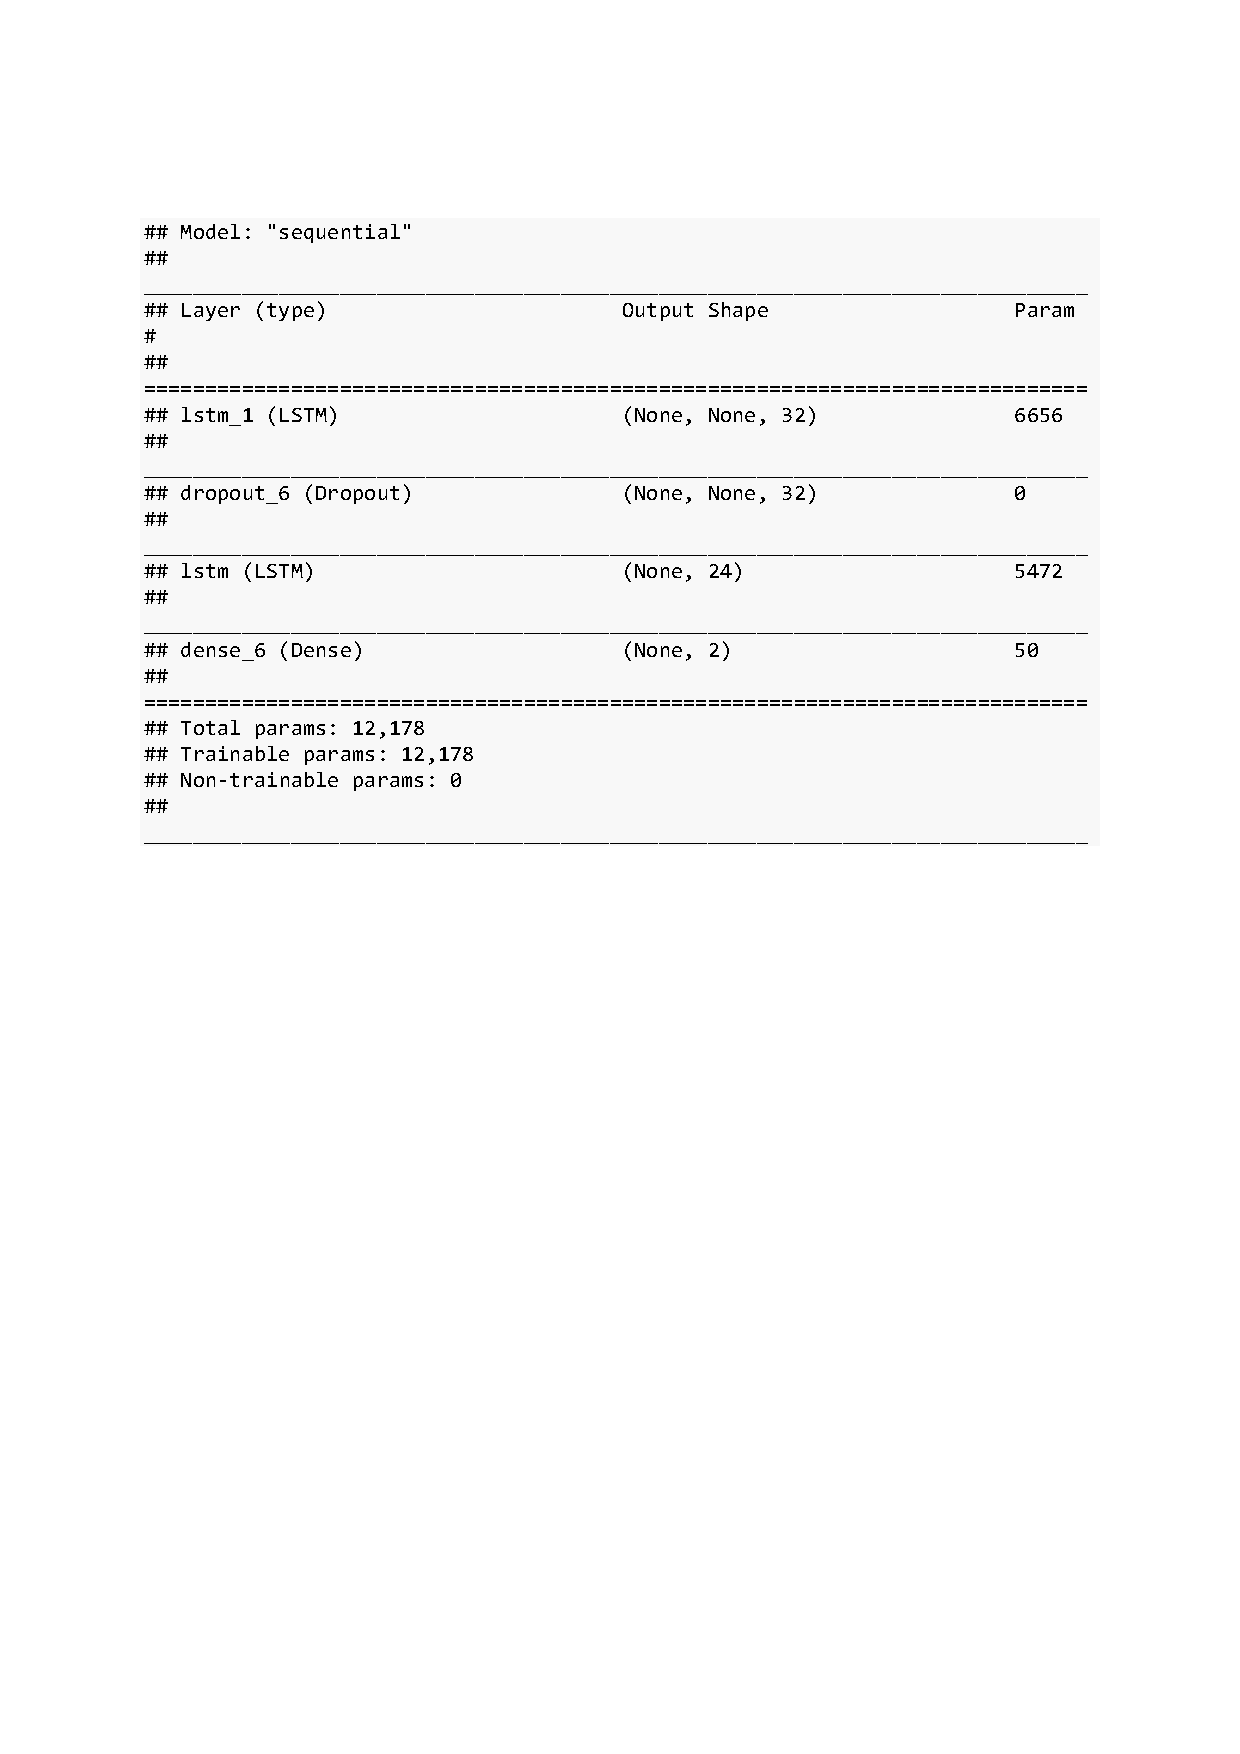
\includegraphics[scale=0.5]{Figures/summary_LSTM_GHL}
	\decoRule
	\caption[Experiment 3: Summary of LSTM for unsupervised learning]{Summary of LSTM \parencite{own}}
	\label{fig:summary_LSTM_GHL}
\end{figure}